\section{Benutzerschnittstelle}
\begin{figure}
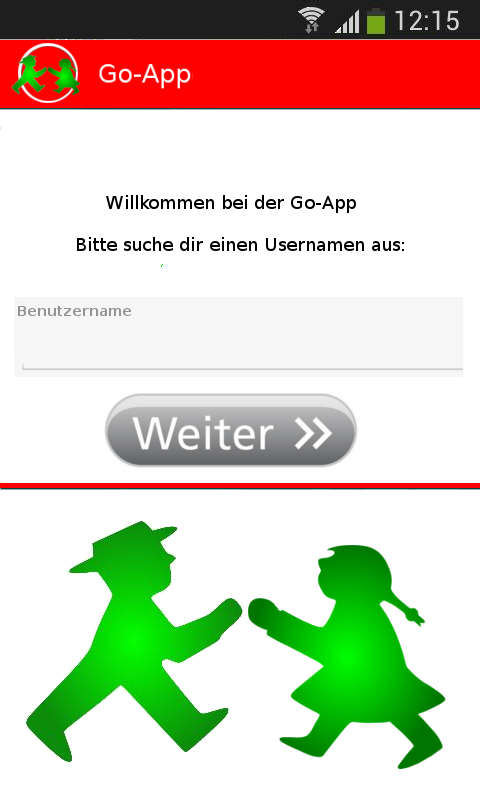
\includegraphics[scale =1]{resources/images/startansicht.png}
\end{figure}
[Bildüberschrift]Erste Startartansicht// //
[Kleinüberschrift]Beschreibung://
Erste Startansicht der App, Begrüßung des neuen Benutzers und Aufforderung sich einen Benutzernamen zu wählen.//
[Kleinüberschrift]Elemente://
Textfeld "User name" zum Einfügen des Benutzernamens//
"Weiter"-Button um diesen zu bestätigen//
[Kleinüberschrift]Verwendung://
Durch einmaliges Tippen auf das Textfeld "User name" wird die Bildschirmtastatur aktiviert und der Benutzer kann seinen gewählten Benutzernamen eintippen.//
Durch einmaliges Tippen auf den "Weiter"-Button wird dieser Benutzername bestätigt und der Benutzer wird weiter geleitet zu der Gruppenübersicht// //

\begin{figure}
	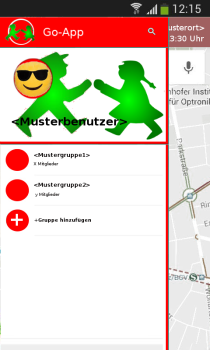
\includegraphics[scale =1]{resources/images/gruppenuebersicht.png}
\end{figure}
[Bildüberschrift]Gruppenübersicht// //
[Kleinüberschrift]Beschreibung://
Übersicht über die Gruppen, in denen der Benutzer Mitglied ist. Wenn der Benutzer das erste Mal zu dieser Ansicht gelangt, ist er in noch keiner Gruppe Mitglied und somit werden ihm auch noch keine angezeigt//
[Kleinüberschrift]Elemente://
Benutzernahme zur Orientierung, wie der Benutzer angemeldet ist//
Gruppennamen zur Übersicht über die Gruppen, in denen der Benutzer Mitglied ist//
"Gruppe hinzufügen"-Button um eine neue Gruppe hinzuzufügen
[Kleinüberschrift]Verwendung://
Blabla noch nicht fertig// //
